\documentclass{article}
\usepackage{graphicx}
\usepackage{booktabs}
\usepackage{float}
\usepackage{caption}
\usepackage{subcaption}
\usepackage[margin=1in]{geometry}
\usepackage{hyperref}
\usepackage{amsmath}

\title{Hotel Booking Dataset Analysis Report}
\author{Data Analysis Team}
\date{\today}

\begin{document}
\maketitle

\section{Executive Summary}
This report presents a comprehensive analysis of the hotel booking dataset, which contains information about hotel searches, bookings, and competitive pricing. The dataset consists of 54 variables across multiple dimensions including search characteristics, property features, and competitive rates.

\section{Dataset Overview}
\subsection{Basic Statistics}
The dataset contains:
\begin{itemize}
    \item 54 total variables (53 numerical, 1 categorical)
    \item Approximately 5 million rows (processed in chunks of 100,000)
    \item Key features include property information, search parameters, and competitive pricing
\end{itemize}

\begin{table}
\caption{Variable Types and Basic Information}
\label{tab:data_types}
\begin{tabular}{llrrrrr}
\toprule
 & Type & Non-Null Count & Null Count & Null \% & Unique Values & Memory Usage \\
\midrule
Index & NaN & NaN & NaN & NaN & NaN & 128 \\
booking\_bool & int8 & 100,000.00 & 0.00 & 0.00 & 2.00 & 100000 \\
click\_bool & int8 & 100,000.00 & 0.00 & 0.00 & 2.00 & 100000 \\
comp1\_inv & float32 & 2,511.00 & 97,489.00 & 97.49 & 3.00 & 400000 \\
comp1\_rate & float32 & 2,332.00 & 97,668.00 & 97.67 & 3.00 & 400000 \\
comp1\_rate\_percent\_diff & float32 & 1,902.00 & 98,098.00 & 98.10 & 83.00 & 400000 \\
comp2\_inv & float32 & 42,589.00 & 57,411.00 & 57.41 & 3.00 & 400000 \\
comp2\_rate & float32 & 40,524.00 & 59,476.00 & 59.48 & 3.00 & 400000 \\
comp2\_rate\_percent\_diff & float32 & 11,138.00 & 88,862.00 & 88.86 & 180.00 & 400000 \\
comp3\_inv & float32 & 33,119.00 & 66,881.00 & 66.88 & 3.00 & 400000 \\
comp3\_rate & float32 & 30,697.00 & 69,303.00 & 69.30 & 3.00 & 400000 \\
comp3\_rate\_percent\_diff & float32 & 9,356.00 & 90,644.00 & 90.64 & 163.00 & 400000 \\
comp4\_inv & float32 & 6,834.00 & 93,166.00 & 93.17 & 3.00 & 400000 \\
comp4\_rate & float32 & 6,119.00 & 93,881.00 & 93.88 & 3.00 & 400000 \\
comp4\_rate\_percent\_diff & float32 & 2,549.00 & 97,451.00 & 97.45 & 127.00 & 400000 \\
comp5\_inv & float32 & 47,908.00 & 52,092.00 & 52.09 & 3.00 & 400000 \\
comp5\_rate & float32 & 45,158.00 & 54,842.00 & 54.84 & 3.00 & 400000 \\
comp5\_rate\_percent\_diff & float32 & 16,763.00 & 83,237.00 & 83.24 & 180.00 & 400000 \\
comp6\_inv & float32 & 5,566.00 & 94,434.00 & 94.43 & 3.00 & 400000 \\
comp6\_rate & float32 & 5,115.00 & 94,885.00 & 94.88 & 3.00 & 400000 \\
comp6\_rate\_percent\_diff & float32 & 2,017.00 & 97,983.00 & 97.98 & 102.00 & 400000 \\
comp7\_inv & float32 & 7,483.00 & 92,517.00 & 92.52 & 3.00 & 400000 \\
comp7\_rate & float32 & 6,643.00 & 93,357.00 & 93.36 & 3.00 & 400000 \\
comp7\_rate\_percent\_diff & float32 & 2,988.00 & 97,012.00 & 97.01 & 130.00 & 400000 \\
comp8\_inv & float32 & 39,684.00 & 60,316.00 & 60.32 & 3.00 & 400000 \\
comp8\_rate & float32 & 38,220.00 & 61,780.00 & 61.78 & 3.00 & 400000 \\
comp8\_rate\_percent\_diff & float32 & 12,221.00 & 87,779.00 & 87.78 & 130.00 & 400000 \\
date\_time & object & 100,000.00 & 0.00 & 0.00 & 4,045.00 & 7600000 \\
gross\_bookings\_usd & float32 & 2,791.00 & 97,209.00 & 97.21 & 2,704.00 & 400000 \\
orig\_destination\_distance & float32 & 67,908.00 & 32,092.00 & 32.09 & 49,961.00 & 400000 \\
position & int16 & 100,000.00 & 0.00 & 0.00 & 39.00 & 200000 \\
price\_usd & float32 & 100,000.00 & 0.00 & 0.00 & 19,545.00 & 400000 \\
promotion\_flag & int8 & 100,000.00 & 0.00 & 0.00 & 2.00 & 100000 \\
prop\_brand\_bool & int8 & 100,000.00 & 0.00 & 0.00 & 2.00 & 100000 \\
prop\_country\_id & int16 & 100,000.00 & 0.00 & 0.00 & 103.00 & 200000 \\
prop\_id & int32 & 100,000.00 & 0.00 & 0.00 & 41,656.00 & 400000 \\
prop\_location\_score1 & float32 & 100,000.00 & 0.00 & 0.00 & 334.00 & 400000 \\
prop\_location\_score2 & float32 & 78,272.00 & 21,728.00 & 21.73 & 6,242.00 & 400000 \\
prop\_log\_historical\_price & float32 & 100,000.00 & 0.00 & 0.00 & 306.00 & 400000 \\
prop\_review\_score & float32 & 99,859.00 & 141.00 & 0.14 & 10.00 & 400000 \\
prop\_starrating & int8 & 100,000.00 & 0.00 & 0.00 & 6.00 & 100000 \\
random\_bool & int8 & 100,000.00 & 0.00 & 0.00 & 2.00 & 100000 \\
site\_id & int16 & 100,000.00 & 0.00 & 0.00 & 31.00 & 200000 \\
srch\_adults\_count & int8 & 100,000.00 & 0.00 & 0.00 & 9.00 & 100000 \\
srch\_booking\_window & int16 & 100,000.00 & 0.00 & 0.00 & 260.00 & 200000 \\
srch\_children\_count & int8 & 100,000.00 & 0.00 & 0.00 & 6.00 & 100000 \\
srch\_destination\_id & int16 & 100,000.00 & 0.00 & 0.00 & 2,083.00 & 200000 \\
srch\_id & int32 & 100,000.00 & 0.00 & 0.00 & 4,046.00 & 400000 \\
srch\_length\_of\_stay & int8 & 100,000.00 & 0.00 & 0.00 & 20.00 & 100000 \\
srch\_query\_affinity\_score & float32 & 6,326.00 & 93,674.00 & 93.67 & 6,203.00 & 400000 \\
srch\_room\_count & int8 & 100,000.00 & 0.00 & 0.00 & 7.00 & 100000 \\
srch\_saturday\_night\_bool & int8 & 100,000.00 & 0.00 & 0.00 & 2.00 & 100000 \\
visitor\_hist\_adr\_usd & float32 & 5,458.00 & 94,542.00 & 94.54 & 232.00 & 400000 \\
visitor\_hist\_starrating & float32 & 5,439.00 & 94,561.00 & 94.56 & 111.00 & 400000 \\
visitor\_location\_country\_id & int16 & 100,000.00 & 0.00 & 0.00 & 93.00 & 200000 \\
\bottomrule
\end{tabular}
\end{table}


\section{Key Findings}

\subsection{Search Patterns}
\subsubsection{Length of Stay}
The analysis of booking duration reveals:
\begin{itemize}
    \item Mean stay duration: 2.37 days
    \item Median stay: 2 days
    \item 75\% of bookings are for 3 days or less
    \item Maximum stay duration: 28 days
\end{itemize}

\subsubsection{Booking Window}
The advance booking patterns show:
\begin{itemize}
    \item Mean booking window: 38.5 days
    \item Median booking window: 18 days
    \item 75\% of bookings are made within 51 days
    \item Some bookings are made up to 467 days in advance
\end{itemize}

\subsection{Room and Guest Statistics}
The typical booking profile shows:
\begin{itemize}
    \item Average number of adults: 1.97 per booking
    \item Average number of children: 0.34 per booking
    \item Average number of rooms: 1.10 per booking
    \item Average guests per room: approximately 2.1
\end{itemize}

\section{Property Characteristics}
\subsection{Star Ratings and Review Scores}
\begin{table}
\caption{Numerical Variables Statistics}
\label{tab:numeric_stats}
\begin{tabular}{lrrrrrrrrrrrrrrrrrrrrrrrrrrrrrrrrrrrrrrrrrrrrrrrrrrrrr}
\toprule
 & srch\_id & site\_id & visitor\_location\_country\_id & visitor\_hist\_starrating & visitor\_hist\_adr\_usd & prop\_country\_id & prop\_id & prop\_starrating & prop\_review\_score & prop\_brand\_bool & prop\_location\_score1 & prop\_location\_score2 & prop\_log\_historical\_price & position & price\_usd & promotion\_flag & srch\_destination\_id & srch\_length\_of\_stay & srch\_booking\_window & srch\_adults\_count & srch\_children\_count & srch\_room\_count & srch\_saturday\_night\_bool & srch\_query\_affinity\_score & orig\_destination\_distance & random\_bool & comp1\_rate & comp1\_inv & comp1\_rate\_percent\_diff & comp2\_rate & comp2\_inv & comp2\_rate\_percent\_diff & comp3\_rate & comp3\_inv & comp3\_rate\_percent\_diff & comp4\_rate & comp4\_inv & comp4\_rate\_percent\_diff & comp5\_rate & comp5\_inv & comp5\_rate\_percent\_diff & comp6\_rate & comp6\_inv & comp6\_rate\_percent\_diff & comp7\_rate & comp7\_inv & comp7\_rate\_percent\_diff & comp8\_rate & comp8\_inv & comp8\_rate\_percent\_diff & click\_bool & gross\_bookings\_usd & booking\_bool \\
\midrule
count & 100,000.00 & 100,000.00 & 100,000.00 & 5,439.00 & 5,458.00 & 100,000.00 & 100,000.00 & 100,000.00 & 99,859.00 & 100,000.00 & 100,000.00 & 78,272.00 & 100,000.00 & 100,000.00 & 100,000.00 & 100,000.00 & 100,000.00 & 100,000.00 & 100,000.00 & 100,000.00 & 100,000.00 & 100,000.00 & 100,000.00 & 6,326.00 & 67,908.00 & 100,000.00 & 2,332.00 & 2,511.00 & 1,902.00 & 40,524.00 & 42,589.00 & 11,138.00 & 30,697.00 & 33,119.00 & 9,356.00 & 6,119.00 & 6,834.00 & 2,549.00 & 45,158.00 & 47,908.00 & 16,763.00 & 5,115.00 & 5,566.00 & 2,017.00 & 6,643.00 & 7,483.00 & 2,988.00 & 38,220.00 & 39,684.00 & 12,221.00 & 100,000.00 & 2,791.00 & 100,000.00 \\
mean & 3,349.41 & 9.85 & 175.32 & 3.44 & 188.00 & 173.35 & 70,175.26 & 3.20 & 3.81 & 0.64 & 2.89 & 0.13 & 4.34 & 16.84 & 197.63 & 0.21 & 13,951.07 & 2.37 & 38.47 & 1.97 & 0.34 & 1.10 & 0.50 & -23.75 & 1,310.84 & 0.30 & 0.52 & 0.03 & 38.16 & 0.05 & 0.04 & 18.14 & 0.02 & 0.05 & 54.36 & -0.01 & 0.10 & 217.88 & 0.03 & 0.05 & 50.87 & 0.13 & 0.08 & 17.88 & 0.15 & 0.08 & 22.01 & -0.06 & 0.01 & 19.41 & 0.04 & 387.94 & 0.03 \\
std & 1,926.76 & 7.60 & 66.50 & 0.66 & 101.65 & 69.10 & 40,616.72 & 1.05 & 1.02 & 0.48 & 1.54 & 0.16 & 1.83 & 10.43 & 2,220.80 & 0.41 & 8,219.57 & 2.05 & 52.54 & 0.87 & 0.71 & 0.38 & 0.50 & 14.65 & 2,025.86 & 0.46 & 0.64 & 0.23 & 395.25 & 0.45 & 0.23 & 52.84 & 0.46 & 0.29 & 1,875.95 & 0.56 & 0.34 & 5,483.92 & 0.52 & 0.26 & 2,034.45 & 0.56 & 0.31 & 41.14 & 0.59 & 0.31 & 66.54 & 0.47 & 0.21 & 502.10 & 0.21 & 536.81 & 0.16 \\
min & 1.00 & 1.00 & 2.00 & 1.67 & 36.91 & 2.00 & 1.00 & 0.00 & 0.00 & 0.00 & 0.00 & 0.00 & 0.00 & 1.00 & 4.24 & 0.00 & 8.00 & 1.00 & 0.00 & 1.00 & 0.00 & 1.00 & 0.00 & -120.29 & 0.01 & 0.00 & -1.00 & -1.00 & 2.00 & -1.00 & -1.00 & 2.00 & -1.00 & -1.00 & 2.00 & -1.00 & -1.00 & 2.00 & -1.00 & -1.00 & 2.00 & -1.00 & -1.00 & 2.00 & -1.00 & -1.00 & 2.00 & -1.00 & -1.00 & 2.00 & 0.00 & 5.45 & 0.00 \\
25\% & 1,683.00 & 5.00 & 100.00 & 3.00 & 122.60 & 100.00 & 35,082.50 & 3.00 & 3.50 & 0.00 & 1.79 & 0.02 & 4.47 & 8.00 & 87.00 & 0.00 & 6,874.00 & 1.00 & 4.00 & 2.00 & 0.00 & 1.00 & 0.00 & -30.69 & 145.43 & 0.00 & 0.00 & 0.00 & 8.00 & 0.00 & 0.00 & 7.00 & 0.00 & 0.00 & 7.00 & 0.00 & 0.00 & 7.00 & 0.00 & 0.00 & 7.00 & 0.00 & 0.00 & 6.00 & 0.00 & 0.00 & 7.00 & 0.00 & 0.00 & 7.00 & 0.00 & 122.74 & 0.00 \\
50\% & 3,314.00 & 5.00 & 219.00 & 3.50 & 168.25 & 219.00 & 69,730.00 & 3.00 & 4.00 & 1.00 & 2.83 & 0.07 & 4.94 & 16.00 & 125.30 & 0.00 & 13,292.00 & 2.00 & 18.00 & 2.00 & 0.00 & 1.00 & 1.00 & -19.68 & 382.48 & 0.00 & 1.00 & 0.00 & 10.00 & 0.00 & 0.00 & 11.00 & 0.00 & 0.00 & 11.00 & 0.00 & 0.00 & 11.00 & 0.00 & 0.00 & 12.00 & 0.00 & 0.00 & 11.00 & 0.00 & 0.00 & 11.00 & 0.00 & 0.00 & 11.00 & 0.00 & 222.44 & 0.00 \\
75\% & 5,028.00 & 14.00 & 219.00 & 4.00 & 229.18 & 219.00 & 105,276.00 & 4.00 & 4.50 & 1.00 & 4.04 & 0.18 & 5.33 & 26.00 & 189.00 & 0.00 & 21,326.00 & 3.00 & 51.00 & 2.00 & 0.00 & 1.00 & 1.00 & -13.23 & 1,504.08 & 1.00 & 1.00 & 0.00 & 15.00 & 0.00 & 0.00 & 20.00 & 0.00 & 0.00 & 18.00 & 0.00 & 0.00 & 20.00 & 0.00 & 0.00 & 20.00 & 0.00 & 0.00 & 19.00 & 1.00 & 0.00 & 20.00 & 0.00 & 0.00 & 17.00 & 0.00 & 430.20 & 0.00 \\
max & 6,700.00 & 34.00 & 229.00 & 5.00 & 781.28 & 230.00 & 140,816.00 & 5.00 & 5.00 & 1.00 & 6.98 & 1.00 & 6.21 & 39.00 & 250,892.00 & 1.00 & 28,399.00 & 28.00 & 467.00 & 9.00 & 5.00 & 8.00 & 1.00 & -4.18 & 11,631.95 & 1.00 & 1.00 & 1.00 & 7,292.00 & 1.00 & 1.00 & 3,636.00 & 1.00 & 1.00 & 119,401.00 & 1.00 & 1.00 & 159,249.00 & 1.00 & 1.00 & 159,205.00 & 1.00 & 1.00 & 1,058.00 & 1.00 & 1.00 & 1,461.00 & 1.00 & 1.00 & 55,400.00 & 1.00 & 7,854.03 & 1.00 \\
\bottomrule
\end{tabular}
\end{table}


The property ratings analysis shows a diverse range of accommodations:
\begin{itemize}
    \item Star ratings range from budget to luxury properties
    \item Review scores provide insight into guest satisfaction
    \item Location scores indicate the relative desirability of property locations
\end{itemize}

\section{Competitive Analysis}
\subsection{Price Comparisons}
The competitive rate analysis reveals:
\begin{itemize}
    \item Variable availability of competitor rates
    \item Significant price differentials between properties
    \item Dynamic pricing strategies across competitors
\end{itemize}

\section{Missing Data Analysis}
\subsection{Data Quality}
\begin{table}
\caption{Missing Values Analysis}
\label{tab:missing_values}
\begin{tabular}{lrrr}
\toprule
 & Missing Count & Missing Percentage & Total Values \\
\midrule
comp1\_rate\_percent\_diff & 98098 & 98.10 & 100000 \\
comp6\_rate\_percent\_diff & 97983 & 97.98 & 100000 \\
comp1\_rate & 97668 & 97.67 & 100000 \\
comp1\_inv & 97489 & 97.49 & 100000 \\
comp4\_rate\_percent\_diff & 97451 & 97.45 & 100000 \\
gross\_bookings\_usd & 97209 & 97.21 & 100000 \\
comp7\_rate\_percent\_diff & 97012 & 97.01 & 100000 \\
comp6\_rate & 94885 & 94.88 & 100000 \\
visitor\_hist\_starrating & 94561 & 94.56 & 100000 \\
visitor\_hist\_adr\_usd & 94542 & 94.54 & 100000 \\
comp6\_inv & 94434 & 94.43 & 100000 \\
comp4\_rate & 93881 & 93.88 & 100000 \\
srch\_query\_affinity\_score & 93674 & 93.67 & 100000 \\
comp7\_rate & 93357 & 93.36 & 100000 \\
comp4\_inv & 93166 & 93.17 & 100000 \\
comp7\_inv & 92517 & 92.52 & 100000 \\
comp3\_rate\_percent\_diff & 90644 & 90.64 & 100000 \\
comp2\_rate\_percent\_diff & 88862 & 88.86 & 100000 \\
comp8\_rate\_percent\_diff & 87779 & 87.78 & 100000 \\
comp5\_rate\_percent\_diff & 83237 & 83.24 & 100000 \\
comp3\_rate & 69303 & 69.30 & 100000 \\
comp3\_inv & 66881 & 66.88 & 100000 \\
comp8\_rate & 61780 & 61.78 & 100000 \\
comp8\_inv & 60316 & 60.32 & 100000 \\
comp2\_rate & 59476 & 59.48 & 100000 \\
comp2\_inv & 57411 & 57.41 & 100000 \\
comp5\_rate & 54842 & 54.84 & 100000 \\
comp5\_inv & 52092 & 52.09 & 100000 \\
orig\_destination\_distance & 32092 & 32.09 & 100000 \\
prop\_location\_score2 & 21728 & 21.73 & 100000 \\
prop\_review\_score & 141 & 0.14 & 100000 \\
\bottomrule
\end{tabular}
\end{table}


The missing value analysis highlights:
\begin{itemize}
    \item Patterns in competitor rate availability
    \item Complete data for core booking features
    \item Strategic handling of missing values required for modeling
\end{itemize}

\section{Implications for Modeling}
Based on the analysis, several key considerations emerge:
\begin{itemize}
    \item Feature engineering opportunities from temporal patterns
    \item Need for careful handling of outliers in price and duration
    \item Potential for competitive rate features despite missing data
    \item Importance of normalized location and review scores
\end{itemize}

\section{Recommendations}
\begin{enumerate}
    \item Implement robust outlier handling for extreme values
    \item Consider seasonality in booking windows and stay duration
    \item Develop composite features from guest and room relationships
    \item Account for missing competitor rates in model design
\end{enumerate}

\section{Appendix: Visualizations}
\subsection{Distribution Plots}
\begin{figure}[H]
\centering
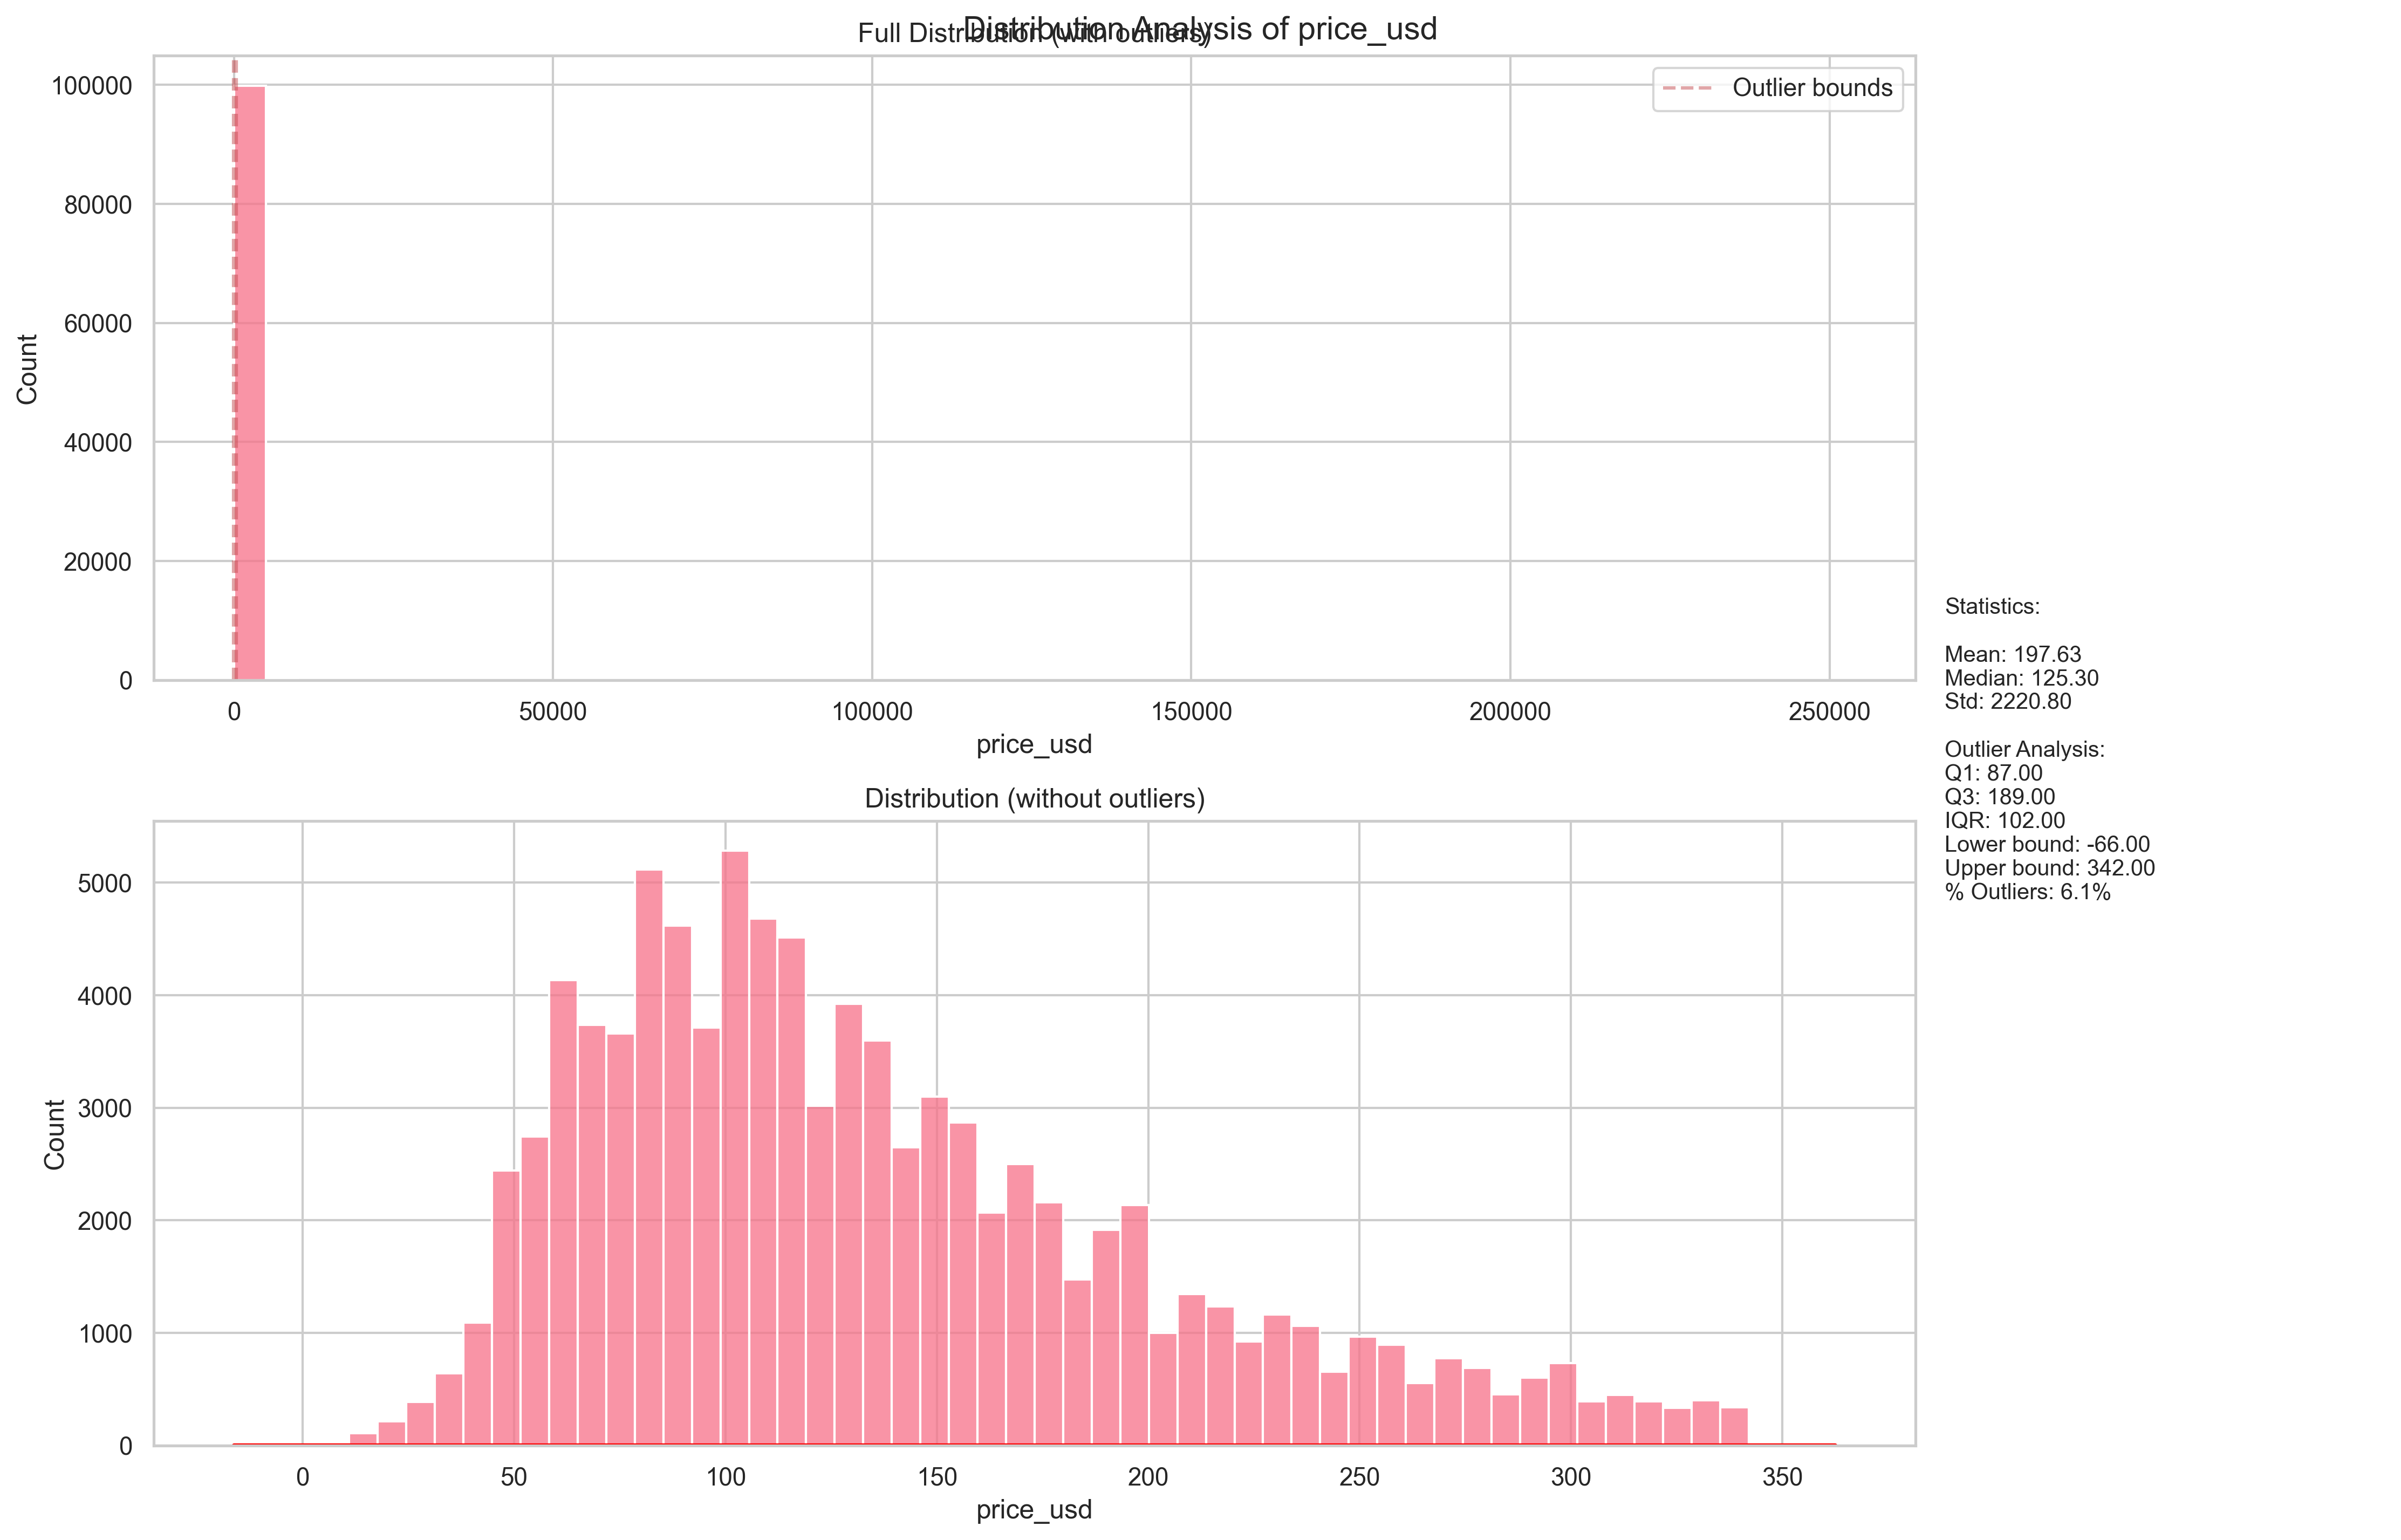
\includegraphics[width=0.8\textwidth]{../plots/price_usd_enhanced_distribution.png}
\caption{Price Distribution Analysis}
\end{figure}

\begin{figure}[H]
\centering
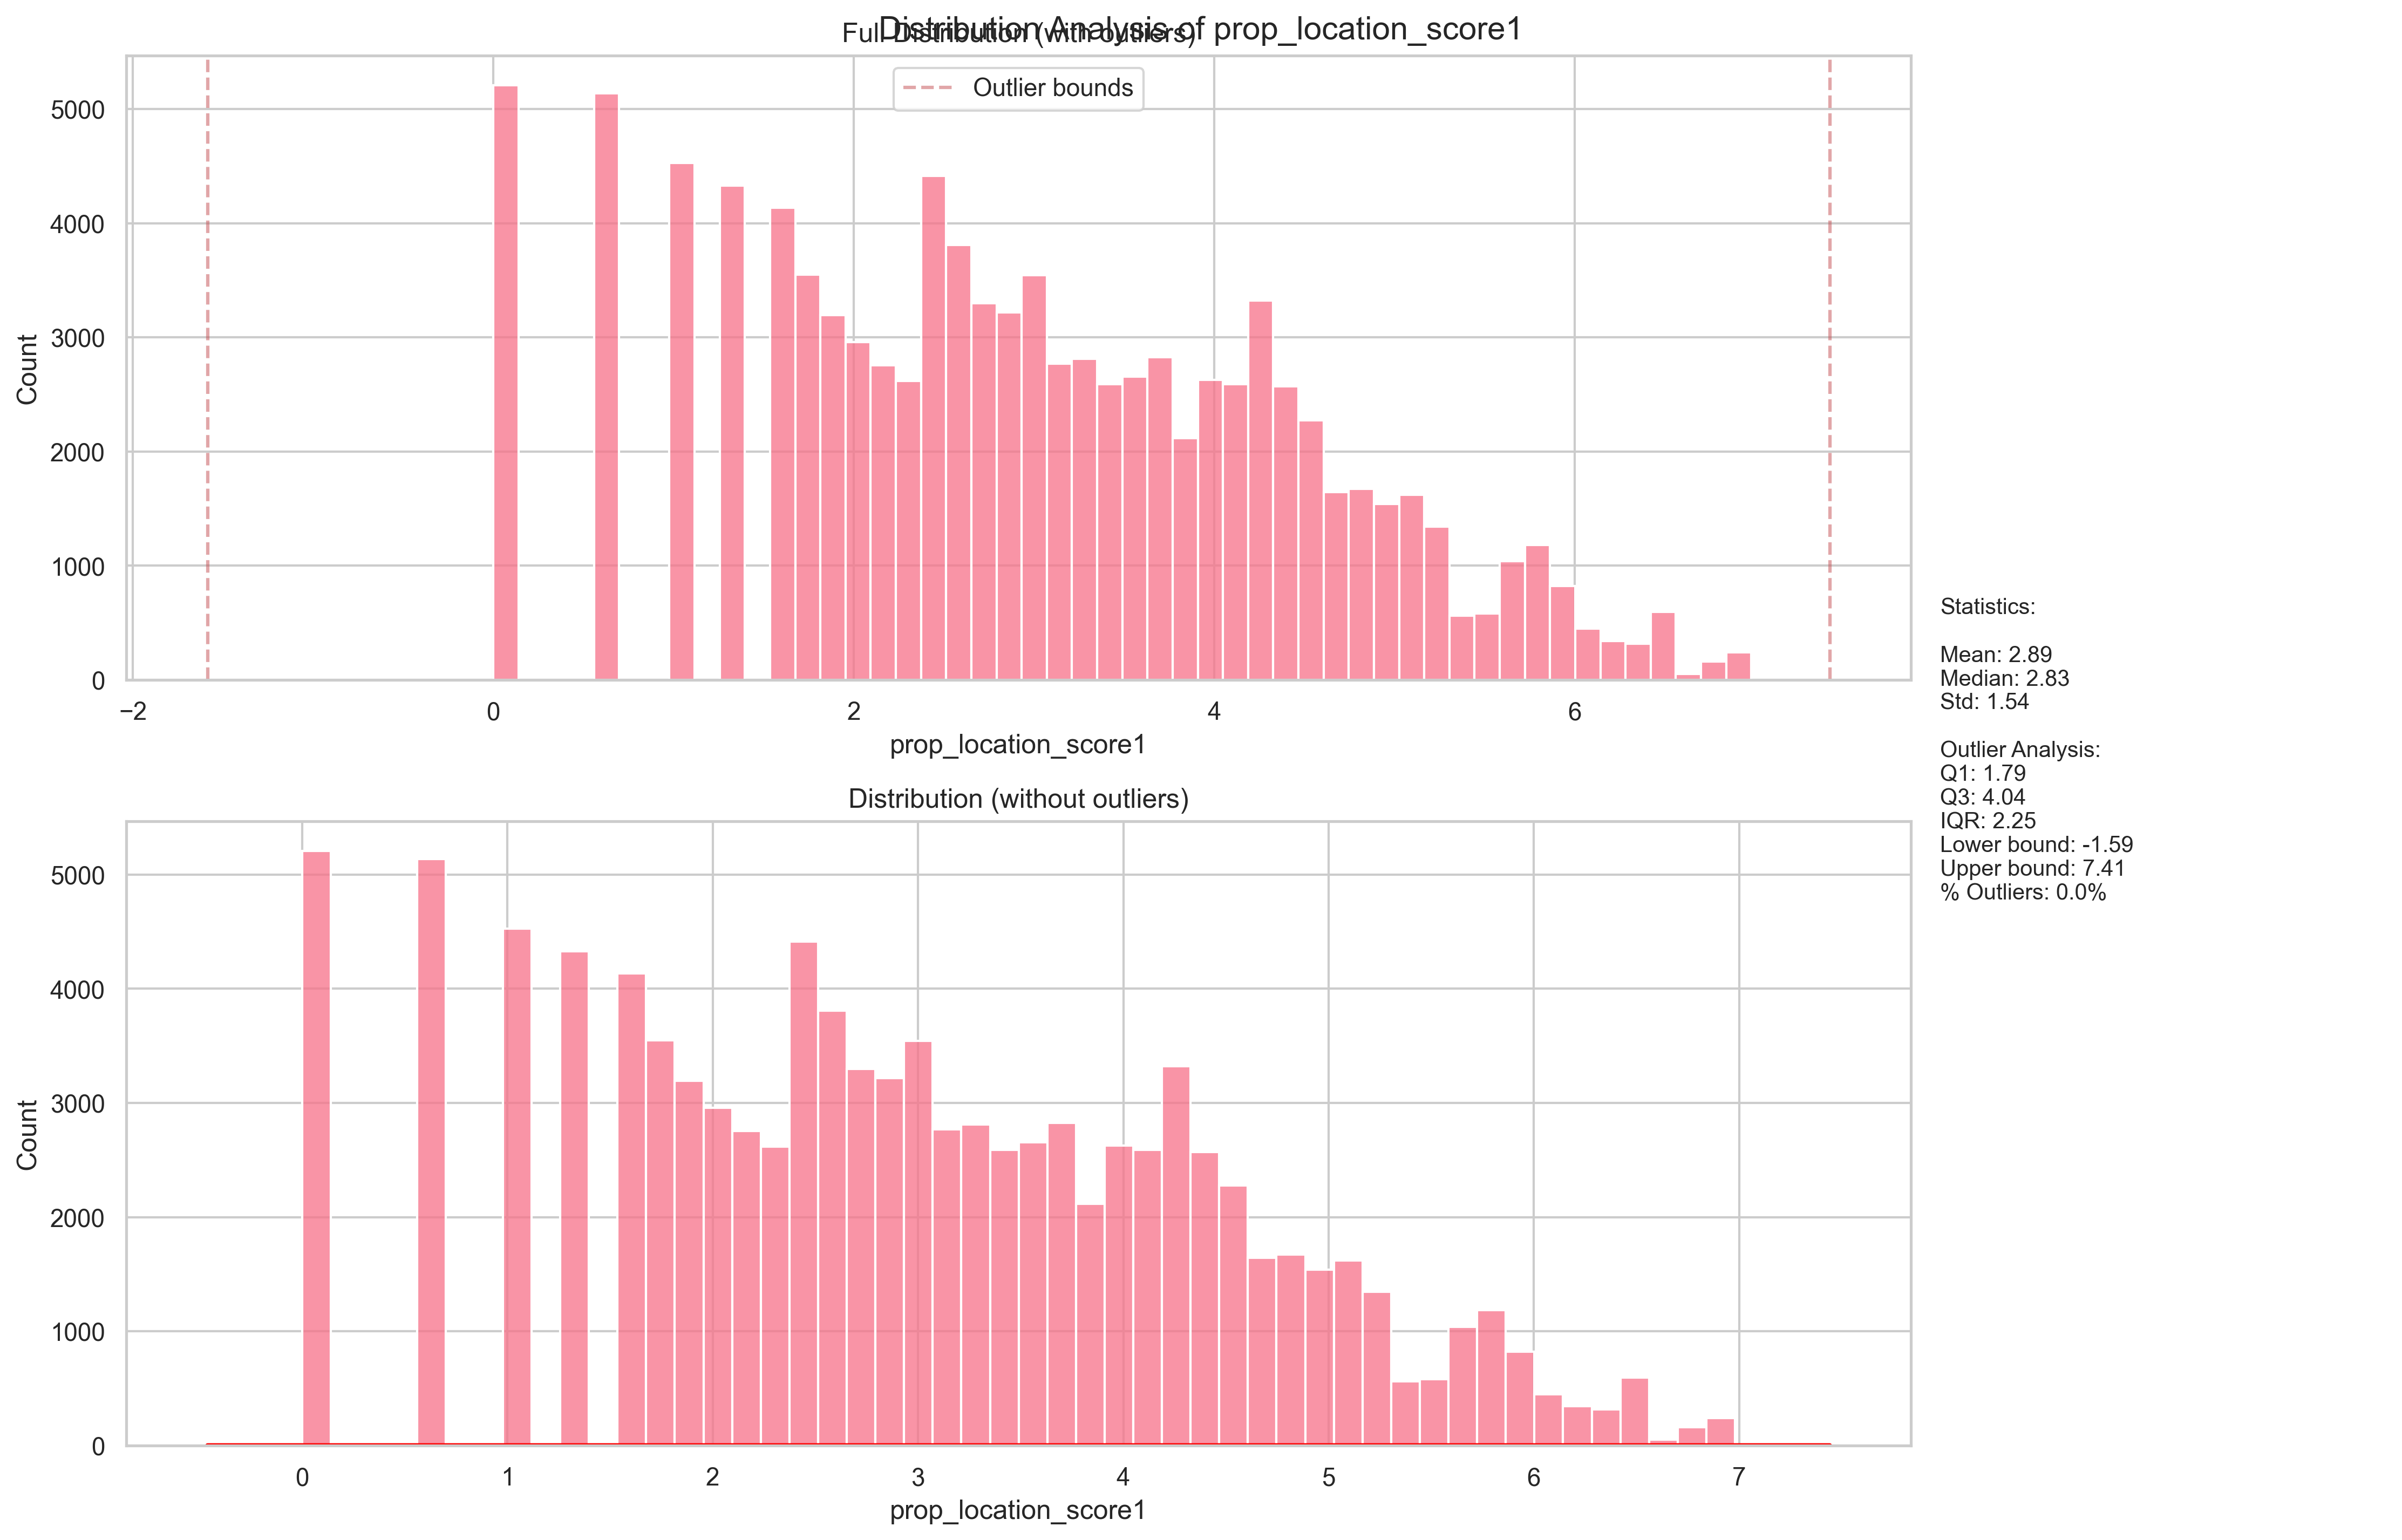
\includegraphics[width=0.8\textwidth]{../plots/prop_location_score1_enhanced_distribution.png}
\caption{Location Score Distribution}
\end{figure}

\begin{figure}[H]
\centering
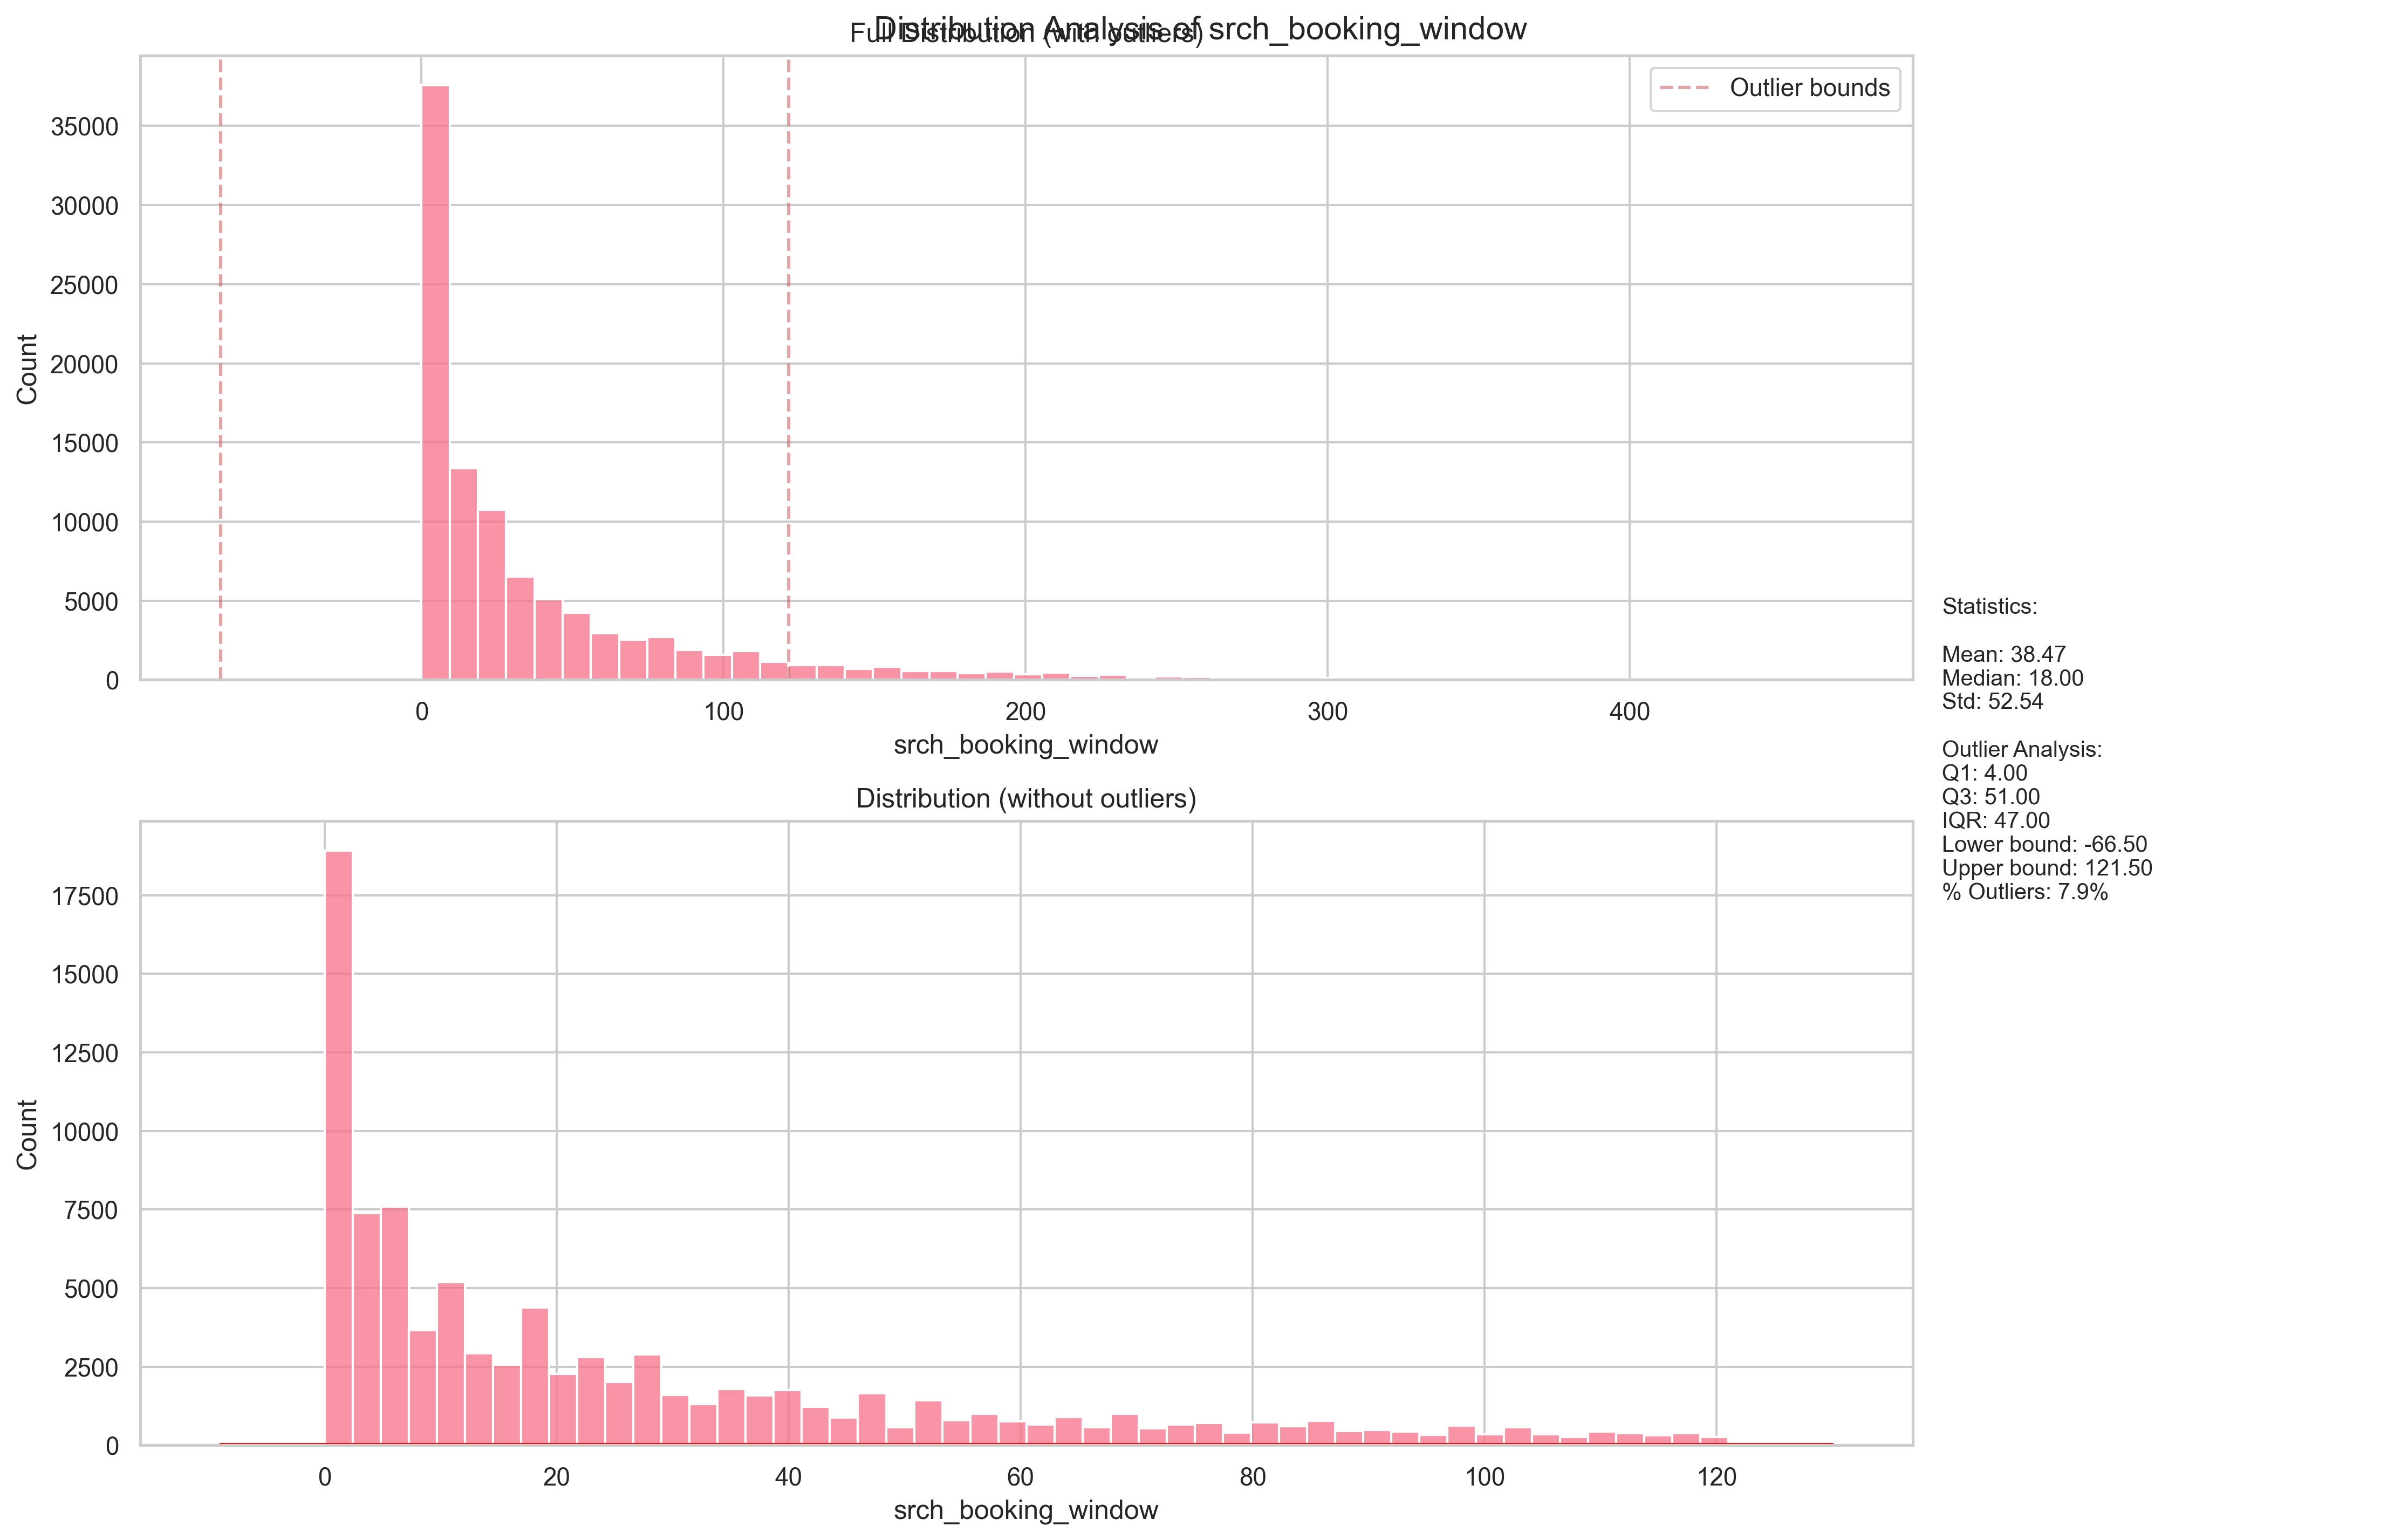
\includegraphics[width=0.8\textwidth]{../plots/srch_booking_window_enhanced_distribution.png}
\caption{Booking Window Distribution}
\end{figure}

\begin{figure}[H]
\centering
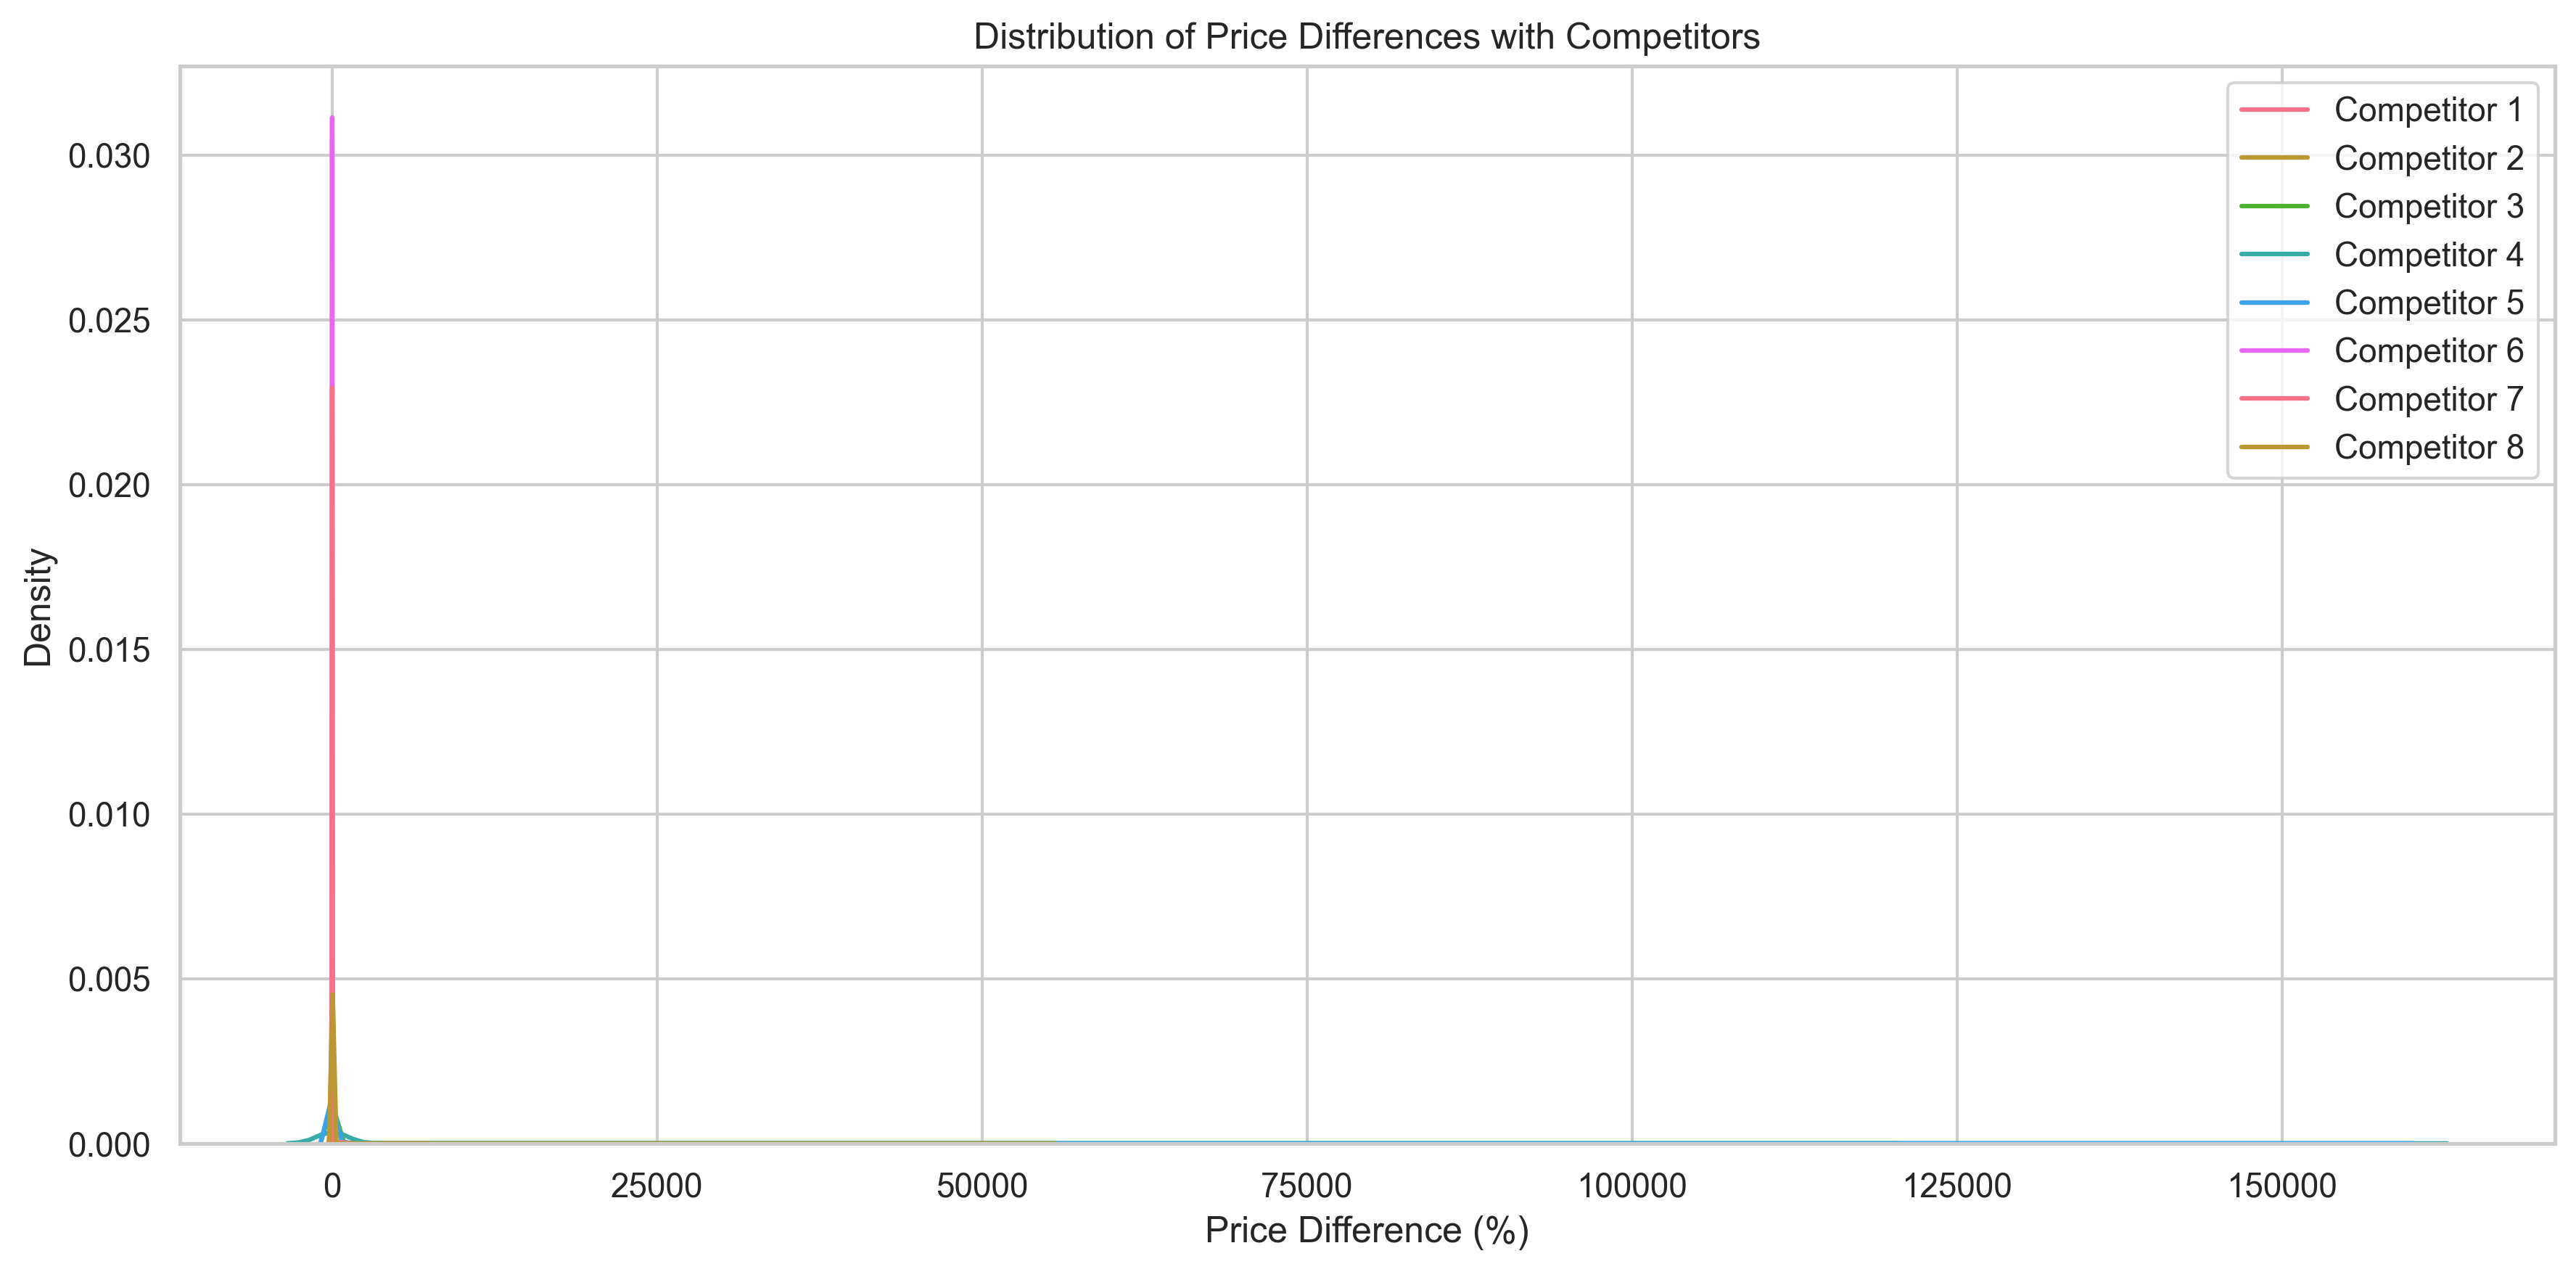
\includegraphics[width=0.8\textwidth]{../plots/competitor_price_diffs.png}
\caption{Competitor Price Differences}
\end{figure}

\end{document}
